% What is a side channel?
In this section, we provide an overview of network side-channel attacks. 
We, further, discuss video streaming as one specific target application of side-channel attacks, and explain the state-of-the-art traffic analysis attack proposed for this application and elaborate on its strengths and weaknesses. 

A side channel is a method of extracting information from a program by observing its functionality and environment, rather than through its intended input or output. 
Extracting information from side channels becomes particularly viable when a program has shared resources with other untrusted entities. 
When an adversary shares resources with the victim's program, it can observe victim's resource usage pattern.
The adversary then can leverage the correlation between resource usage pattern (side channels) and victims' secrets to breach their privacy.

% Essential Steps in side channel attacks
A side-channel attack comprises two essential steps: Profiling and Inference.
During profiling, the adversary extracts the correlation between the victim's secrets and their resource usage patterns.
This involves monitoring various resource usage patterns that emerge during the program's execution.
In the inference step, the adversary utilizes the prior knowledge acquired in the first step to infer the victim's secrets based on the observations of resource usage patterns.
One trivial solution to address side-channel attack is to isolate the program and all its dedicated resources such as CPUs, memory, storage, and network resources at all possible level down to hardware. 
However, this approach often results in inefficient resource utilization, as the resources that the program does not currently use remain idle. 
Moreover, many programs rely on inherently shared resources, such as a common network infrastructure.
Therefore, mitigating side-channels attacks is intrinsically challenging. 

% What are network side channels 
Network applications, such as web browsers, email clients, video conferencing software, file-sharing services, and online gaming platforms, are exceedingly popular these days.
These applications consist of a service that communicates with clients over an encrypted communication on the network.
However, the encryption does not conceal packet sizes and timing transmitted by an application, which is correlated with users' sensitive information in many applications.
In a network side-channel attack, by utilizing this correlation, an adversary with control over the underlying network links (e.g., Internet Service Providers) can monitor the traffic pattern and potentially reveal the content of the communication.
Recent advancements in machine learning have significantly empowered the inference step of network side-channel attacks, providing adversaries with enhanced capabilities to effectively map observations to the victim's sensitive information~\cite{schuster2017beautyburst, bhat2019varcnn, hayes2016kfp, sirinam2018df}.


% \subsection{Website Fingerprinting}\label{subsec:web-fingerprinting}

\subsection{Video identification}\label{subsec:video-classification}
Recently, video services have gained immense popularity, becoming an integral part of people's daily Internet activities.
Video-sharing platforms, such as YouTube, and commercial online streaming platforms, such as Netflix, constitute a significant portion of the world's total network traffic.
In 2023, video services account for 82.5\% of all web traffic, making them by far the most popular type of content over the internet~\cite{webstat}.
The popularity of these services makes them a natural target for traffic analysis attacks.
Video streams are characterized by bursty traffic patterns, which often involves short-lived periods of high rate data transmission interspersed with relatively longer periods of low or moderate rate network activity.
When these patterns are correlated with specific content, an adversary capable of measuring them may have the ability to identify the exact video being streamed.
In this section, we first provide an overview of the widely used video streaming protocol, Dynamic Adaptive Streaming over HTTP (MPEG-DASH), and examine how it can potentially result in information leakage. 
Next, we elaborate on the state-of-the-art network side-channel attack, known as Beauty and the Burst~\cite{schuster2017beautyburst}, which leverages bursty pattern of MPEG-DASH protocol to reveal users' information. 

In MPEG-DASH protocol, the video server encodes the video content and divide it into short segments, ranging from few seconds to few tens of seconds.
Then, it creates a Manifest file to store information about available data segments, their quality, and a URL to access them.
Upon receiving a request for a video from a client, the video server sends the Manifest file to the client. 
Following this, the client sends requests based on the URLs provided in the Manifest file to download segments corresponding to the desired quality.
The segment sizes and the timing of each segment can collectively create a unique pattern for a video.
An adversary with control over network link can measure segment sizes and their temporal pattern to identify the streaming video.
In Beauty and the Burst paper~\cite{schuster2017beautyburst}, the authors show that even a malicious extension in a browser, can extract segment sizes and timing of a video that the user is watching.
Based on the MPEG-DASH standard, Beauty and Burst attack model traffic traces as time-series.
Specifically, each traffic segment can be represented as a tuple $(t_i, b_i)$, where $t_i$ denotes the segment's transmission time and $b_i$ represents its size. 
A traffic analysis attack involves the attempt to infer the content of traffic from its observed pattern, which is essentially a sequence modeling task.
At the inference stage, Beauty and the burst~\cite{schuster2017beautyburst} utilizes a convolutional neural network (CNN) architecture to classify videos based on the time-series representation of observed traffic.
The architecture of Burst and Beauty model is represented in \Cref{fig:bandb-arch}. 
We evaluate this architecture with our dataset in section \Cref{sec:eval-empirical-privacy}.
\begin{figure}[t]
  \centering
  %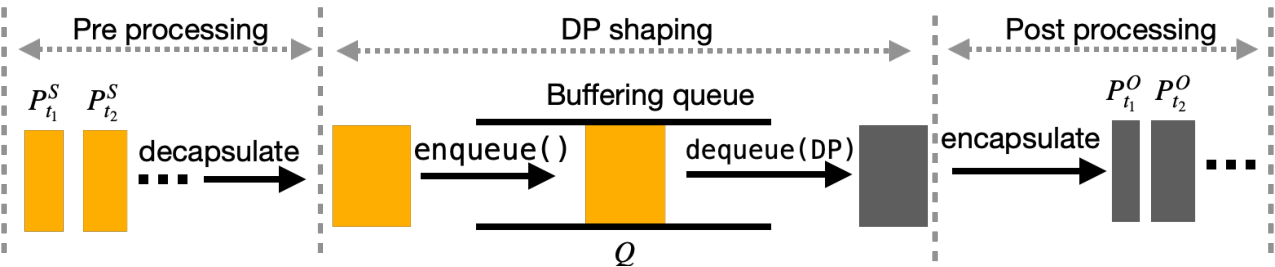
\includegraphics[width=\columnwidth]{figures/DPshaping_concept_vertical.pdf}
  %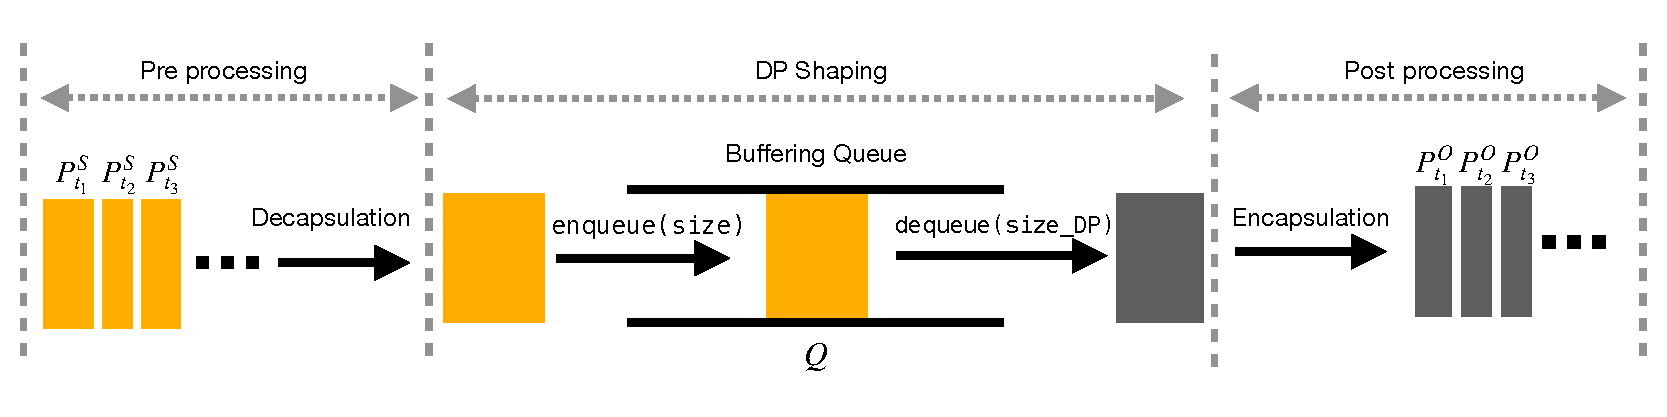
\includegraphics[width=\columnwidth]{figures/DPshaping_concept_horizontal.pdf}
  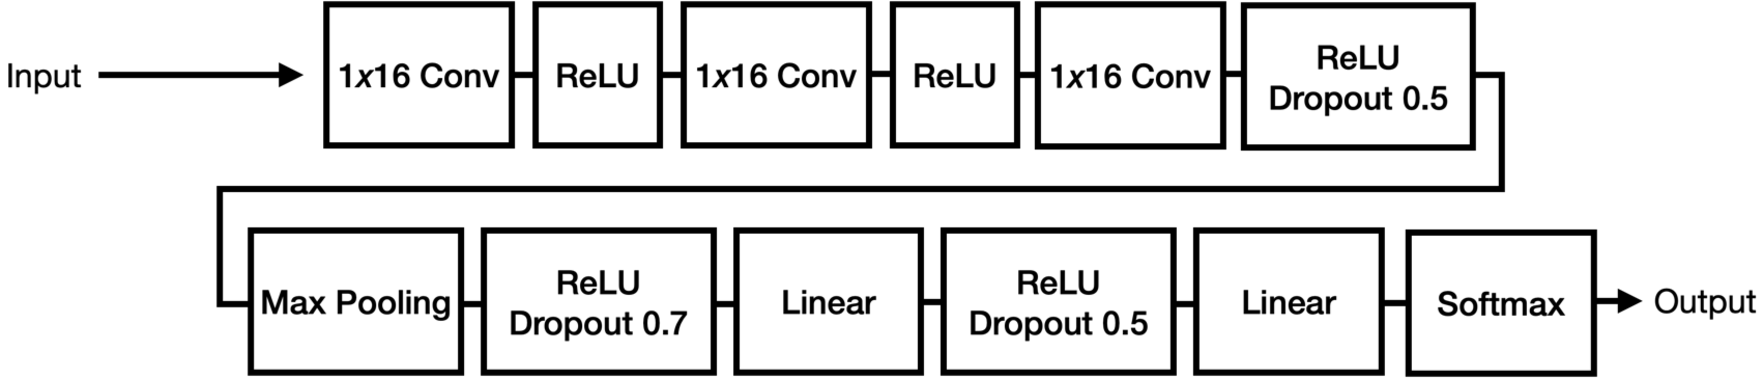
\includegraphics[width=\columnwidth]{figures/BandB_arch.pdf}
  \caption{Beauty and The Burst CNN model architecture.}
  \label{fig:bandb-arch}
\end{figure}

\subsection{Website Fingerprinting}
Website fingerprinting is similar to video identification in essence.
In website fingerprinting attacks, the attacker goal is to map the victim's packet sequence to the website victim visits at the time. 
Deep Neural Networks (DNNs) are shown to be effective in website fingerprinting attacks~\cite{sirinam2018df}.
However, due to the differences in characteristics of website traffic as compared to video streaming applications, website fingerprinting attacks use different set of features and model architectures. 
A notable contrast distinguishing video from web traffic traces is the comparatively shorter duration of web traces as opposed to the more extended durations typical of video traces.
Sirinam~\etalc{sirinam2018df} show that a small CNN with one convolutional layer is able to map users' traffic to their content with 98\% accuracy.
They further show that their model is able to achieve 90\% accuracy in presence of WTF-PAD~\cite{juarez2016wtfpad} defense mechanism, and it achieves 49.7\% accuracy when Walke-Talkie is deployed.
This highlights the ineffectiveness of ad-hoc shaping mechanism in face of emerging attacks.

